% flashcards-title: Three rectangular arrays for twelve
% flashcards-desc: Twelve dots are arranged as one by twelve, two by six, and three by four rectangles.
\documentclass[dvisvgm,tikz,border=8pt]{standalone}
\usetikzlibrary{arrows.meta,patterns}

\definecolor{qraNavy}{HTML}{17324D}
\definecolor{qraBlue}{HTML}{2B6CB0}
\definecolor{qraGold}{HTML}{B7791F}
\definecolor{qraPale}{HTML}{EAF2F8}
\definecolor{qraGray}{HTML}{5C6773}

\tikzset{
  qra axis/.style={draw=qraNavy, line width=1.2pt},
  qra tick/.style={draw=qraNavy, line width=1pt},
  qra guide/.style={draw=qraGray, densely dashed, line width=0.8pt},
  qra counter/.style={circle, draw=qraNavy, fill=qraPale, line width=0.9pt, minimum size=7mm, inner sep=0pt},
  qra label/.style={font=\sffamily\bfseries, text=qraNavy},
  qra small label/.style={font=\sffamily, text=qraNavy},
}

\begin{document}
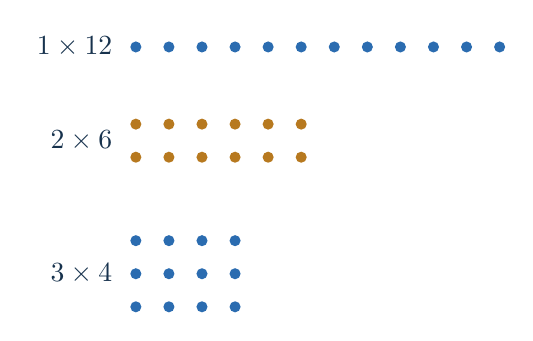
\begin{tikzpicture}[x=.42cm,y=.42cm]
  \foreach \x in {0,...,11}{\fill[qraBlue] (\x,0) circle (2pt);}
  \node[qra label,left=5pt] at (0,0) {$1\times12$};
  \begin{scope}[yshift=-1.4cm]\foreach \x in {0,...,5}{\foreach \y in {0,1}{\fill[qraGold] (\x,\y) circle (2pt);}}\node[qra label,left=5pt] at (0,.5) {$2\times6$};\end{scope}
  \begin{scope}[yshift=-3.3cm]\foreach \x in {0,...,3}{\foreach \y in {0,1,2}{\fill[qraBlue] (\x,\y) circle (2pt);}}\node[qra label,left=5pt] at (0,1) {$3\times4$};\end{scope}
\end{tikzpicture}
\end{document}
